% A LaTeX template for MSc Thesis submissions to 
% Politecnico di Milano (PoliMi) - School of Industrial and Information Engineering
%
% S. Bonetti, A. Gruttadauria, G. Mescolini, A. Zingaro
% e-mail: template-tesi-ingind@polimi.it
%
% Last Revision: October 2021
%
% Copyright 2021 Politecnico di Milano, Italy. NC-BY

\documentclass{Configuration_Files/PoliMi3i_thesis}

%------------------------------------------------------------------------------
%	REQUIRED PACKAGES AND  CONFIGURATIONS
%------------------------------------------------------------------------------

% CONFIGURATIONS
\usepackage{parskip} % For paragraph layout
\usepackage{setspace} % For using single or double spacing
\usepackage{emptypage} % To insert empty pages
\usepackage{multicol} % To write in multiple columns (executive summary)
\setlength\columnsep{15pt} % Column separation in executive summary
\setlength\parindent{0pt} % Indentation
\raggedbottom  

% PACKAGES FOR TITLES
\usepackage{titlesec}
% \titlespacing{\section}{left spacing}{before spacing}{after spacing}
\titlespacing{\section}{0pt}{3.3ex}{2ex}
\titlespacing{\subsection}{0pt}{3.3ex}{1.65ex}
\titlespacing{\subsubsection}{0pt}{3.3ex}{1ex}
\usepackage{color}

% PACKAGES FOR LANGUAGE AND FONT
\usepackage[english]{babel} % The document is in English  
\usepackage[utf8]{inputenc} % UTF8 encoding
\usepackage[T1]{fontenc} % Font encoding
\usepackage[11pt]{moresize} % Big fonts

% PACKAGES FOR IMAGES
\usepackage{graphicx}
\usepackage{transparent} % Enables transparent images
\usepackage{eso-pic} % For the background picture on the title page
\usepackage{subfig} % Numbered and caption subfigures using \subfloat.
\usepackage{tikz} % A package for high-quality hand-made figures.
\usetikzlibrary{}
\graphicspath{{./Images/}} % Directory of the images
\usepackage{caption} % Coloured captions
\usepackage{xcolor} % Coloured captions
\usepackage{amsthm,thmtools,xcolor} % Coloured "Theorem"
\usepackage{float}
\usepackage{listings}

% STANDARD MATH PACKAGES
\usepackage{amsmath}
\usepackage{amsthm}
\usepackage{amssymb}
\usepackage{amsfonts}
\usepackage{bm}
\usepackage[overload]{empheq} % For braced-style systems of equations.
\usepackage{fix-cm} % To override original LaTeX restrictions on sizes

% PACKAGES FOR TABLES
\usepackage{tabularx}
\usepackage{longtable} % Tables that can span several pages
\usepackage{colortbl}

% PACKAGES FOR ALGORITHMS (PSEUDO-CODE)
\usepackage{algorithm}
\usepackage{algorithmic}

% PACKAGES FOR REFERENCES & BIBLIOGRAPHY
\usepackage[colorlinks=true,linkcolor=black,anchorcolor=black,citecolor=black,filecolor=black,menucolor=black,runcolor=black,urlcolor=black]{hyperref} % Adds clickable links at references
\usepackage{cleveref}
\usepackage[square, numbers, sort&compress]{natbib} % Square brackets, citing references with numbers, citations sorted by appearance in the text and compressed
\bibliographystyle{abbrvnat} % You may use a different style adapted to your field

% OTHER PACKAGES
\usepackage{pdfpages} % To include a pdf file
\usepackage{afterpage}
\usepackage{lipsum} % DUMMY PACKAGE
\usepackage{fancyhdr} % For the headers
\fancyhf{}

\definecolor{codegreen}{rgb}{0,0.6,0}
\definecolor{codegray}{rgb}{0.5,0.5,0.5}
\definecolor{codepurple}{rgb}{0.58,0,0.82}
\definecolor{backcolour}{rgb}{0.95,0.95,0.92}

\usepackage{color}

\hypersetup{
colorlinks=true, %set true if you want colored links
linktoc=all,     %set to all if you want both sections and subsections linked
linkcolor=black,  %choose some color if you want links to stand out
urlcolor=blue,
}

\lstdefinestyle{mystyle}{
backgroundcolor=\color{backcolour},
commentstyle=\color{codegreen},
keywordstyle=\color{magenta},
numberstyle=\tiny\color{codegray},
stringstyle=\color{codepurple},
basicstyle=\ttfamily\footnotesize,
breakatwhitespace=false,
breaklines=true,
captionpos=b,
keepspaces=true,
numbers=left,
numbersep=5pt,
showspaces=false,
showstringspaces=false,
showtabs=false,
tabsize=2
}

\lstset{style=mystyle}


% Input of configuration file. Do not change config.tex file unless you really know what you are doing. 
% Define blue color typical of polimi
\definecolor{bluepoli}{cmyk}{0.4,0.1,0,0.4}

% Custom theorem environments
\declaretheoremstyle[
  headfont=\color{bluepoli}\normalfont\bfseries,
  bodyfont=\color{black}\normalfont\itshape,
]{colored}

% Set-up caption colors
\captionsetup[figure]{labelfont={color=bluepoli}} % Set colour of the captions
\captionsetup[table]{labelfont={color=bluepoli}} % Set colour of the captions
\captionsetup[algorithm]{labelfont={color=bluepoli}} % Set colour of the captions

\theoremstyle{colored}
\newtheorem{theorem}{Theorem}[chapter]
\newtheorem{proposition}{Proposition}[chapter]

% Enhances the features of the standard "table" and "tabular" environments.
\newcommand\T{\rule{0pt}{2.6ex}}
\newcommand\B{\rule[-1.2ex]{0pt}{0pt}}

% Pseudo-code algorithm descriptions.
\newcounter{algsubstate}
\renewcommand{\thealgsubstate}{\alph{algsubstate}}
\newenvironment{algsubstates}
  {\setcounter{algsubstate}{0}%
   \renewcommand{\STATE}{%
     \stepcounter{algsubstate}%
     \Statex {\small\thealgsubstate:}\space}}
  {}

% New font size
\newcommand\numfontsize{\@setfontsize\Huge{200}{60}}

% Title format: chapter
\titleformat{\chapter}[hang]{
\fontsize{50}{20}\selectfont\bfseries\filright}{\textcolor{bluepoli} \thechapter\hsp\hspace{2mm}\textcolor{bluepoli}{|   }\hsp}{0pt}{\huge\bfseries \textcolor{bluepoli}
}

% Title format: section
\titleformat{\section}
{\color{bluepoli}\normalfont\Large\bfseries}
{\color{bluepoli}\thesection.}{1em}{}

% Title format: subsection
\titleformat{\subsection}
{\color{bluepoli}\normalfont\large\bfseries}
{\color{bluepoli}\thesubsection.}{1em}{}

% Title format: subsubsection
\titleformat{\subsubsection}
{\color{bluepoli}\normalfont\large\bfseries}
{\color{bluepoli}\thesubsubsection.}{1em}{}

% Shortening for setting no horizontal-spacing
\newcommand{\hsp}{\hspace{0pt}}

\makeatletter
% Renewcommand: cleardoublepage including the background pic
\renewcommand*\cleardoublepage{%
  \clearpage\if@twoside\ifodd\c@page\else
  \null
  \AddToShipoutPicture*{\BackgroundPic}
  \thispagestyle{empty}%
  \newpage
  \if@twocolumn\hbox{}\newpage\fi\fi\fi}
\makeatother

%For correctly numbering algorithms
\numberwithin{algorithm}{chapter}

%----------------------------------------------------------------------------
%	NEW COMMANDS DEFINED
%----------------------------------------------------------------------------

% EXAMPLES OF NEW COMMANDS
\newcommand{\bea}{\begin{eqnarray}} % Shortcut for equation arrays
\newcommand{\eea}{\end{eqnarray}}
\newcommand{\e}[1]{\times 10^{#1}}  % Powers of 10 notation

%----------------------------------------------------------------------------
%	ADD YOUR PACKAGES (be careful of package interaction)
%----------------------------------------------------------------------------

%----------------------------------------------------------------------------
%	ADD YOUR DEFINITIONS AND COMMANDS (be careful of existing commands)
%----------------------------------------------------------------------------

%----------------------------------------------------------------------------
%	BEGIN OF YOUR DOCUMENT
%----------------------------------------------------------------------------

\begin{document}

\fancypagestyle{plain}{%
\fancyhf{} % Clear all header and footer fields
\fancyhead[RO,RE]{\thepage} %RO=right odd, RE=right even
\renewcommand{\headrulewidth}{0pt}
\renewcommand{\footrulewidth}{0pt}}

%----------------------------------------------------------------------------
%	TITLE PAGE
%----------------------------------------------------------------------------

\pagestyle{empty} % No page numbers
\frontmatter % Use roman page numbering style (i, ii, iii, iv...) for the preamble pages

\puttitle{
	title=Systems and Methods for Big and Unstructured Data Project,
	name1=Gabriele Ginestroni, % Author Name and Surname
	name2=Giacomo Gumiero,
	name3=Lorenzo Iovine,
	name4=Nicola Landini,
	name5=Francesco Leone,
	academicyear=2022-2023,
	groupnumber=10
} % These info will be put into your Title page 

%----------------------------------------------------------------------------
%	PREAMBLE PAGES: ABSTRACT (inglese e italiano), EXECUTIVE SUMMARY
%----------------------------------------------------------------------------
\startpreamble
\setcounter{page}{1} % Set page counter to 1

%----------------------------------------------------------------------------
%	LIST OF CONTENTS/FIGURES/TABLES/SYMBOLS
%----------------------------------------------------------------------------

% TABLE OF CONTENTS
\thispagestyle{empty}
\tableofcontents % Table of contents 
\thispagestyle{empty}
\cleardoublepage

%-------------------------------------------------------------------------
%	THESIS MAIN TEXT
%-------------------------------------------------------------------------
% In the main text of your thesis you can write the chapters in two different ways:
%
%(1) As presented in this template you can write:
%    \chapter{Title of the chapter}
%    *body of the chapter*
%
%(2) You can write your chapter in a separated .tex file and then include it in the main file with the following command:
%    \chapter{Title of the chapter}
%    \input{chapter_file.tex}
%
% Especially for long thesis, we recommend you the second option.

\addtocontents{toc}{\vspace{2em}} % Add a gap in the Contents, for aesthetics
\mainmatter % Begin numeric (1,2,3...) page numbering

\chapter{Introduction}
\label{ch:introduction}%
% The \label{...}% enables to remove the small indentation that is generated, always leave the % symbol.

In this chapter will be presented the problem specification and the hypothesis under which the database is implemented.

\section{Problem Specification}
\label{sec:prob_specs}
This project aims to build an Information System that handles scientific articles contained in the DBLP
bibliography. The project involves managing the type of the articles and the associated DOI (Digital Object Identifier),
which identifies a publication or a document and links to it on the web. Other entities to deal with are authors, identified by
an ID or ORCID (Open Researcher and Contributor ID), and their affiliations with organizations. In order to address the
problem, we will store data in a graph database, allowing us to visualize relations and handle information correctly.


\section{Assumptions}
\label{sec:assumptions}
\begin{enumerate}
    \item All the data in the dataset are heterogeneous, so fields are different
    \item The \textbf{authors} with missing field \emph{\_id} are not considered
    \item It is possible that an author writes for different organizations
    \item Field \emph{\_id} in \textbf{author} is unique
    \item Field \emph{\_id} in \textbf{article} exists and it is unique
    \item It is impossible that 2 different articles are on the same journal, in the same \emph{volume} with an intersection between \emph{page\_start} and \emph{page\_end}
    \item The designed model doesn't take into consideration the URL associated to the article node, as the main focus of the project was not reading the article
    \item It is possible to find a self-reference in a publication
    \item A \emph{venue} can be instantiated as a journal, a conference or a generic venue!!!!!!!!
\end{enumerate}

\chapter{ER Diagram}
\begin{figure}[H]
    \centering
    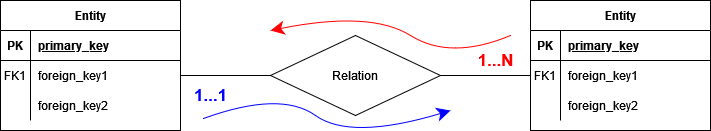
\includegraphics[width=0.6\textwidth]{legendaER.png}
    \caption{ER Diagram Organization}
    \label{fig:erleg}
\end{figure}
\bigskip
\begin{figure}[H]
    \centering
    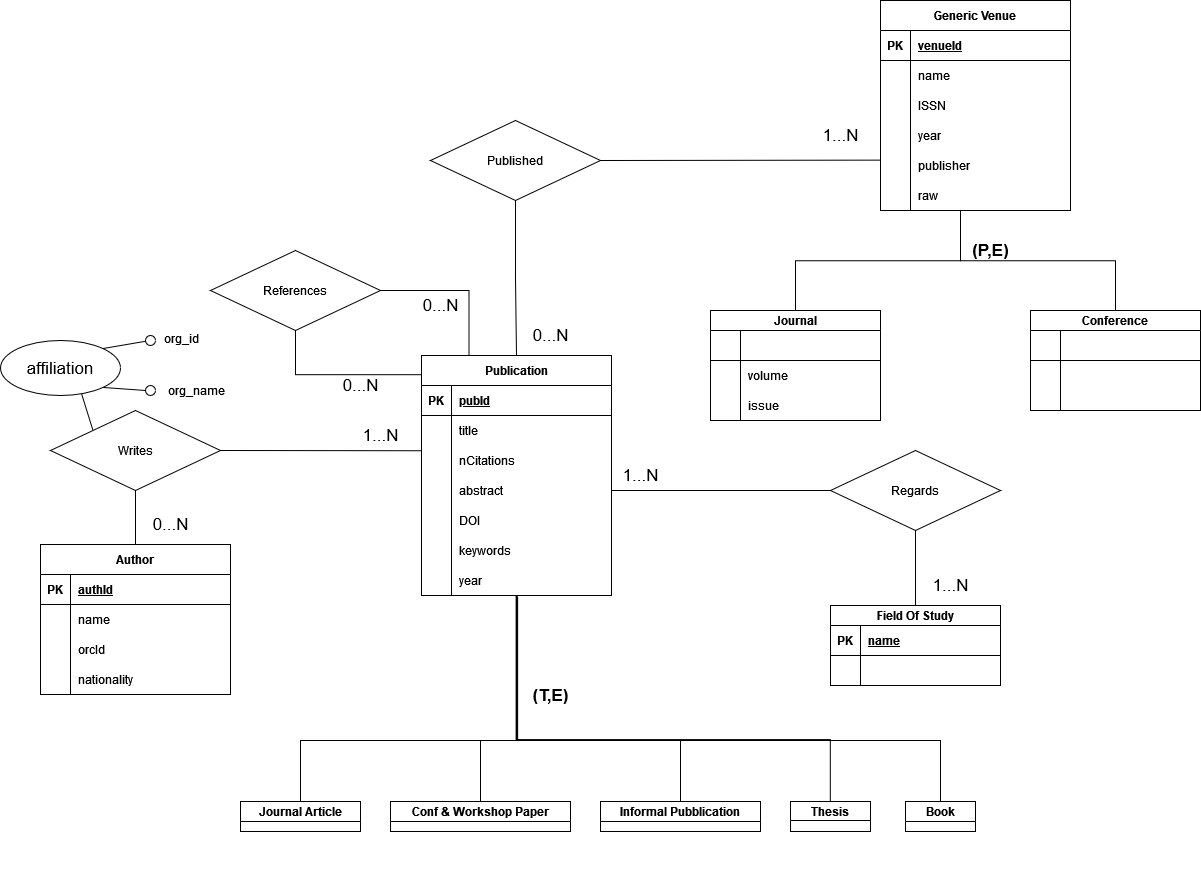
\includegraphics[width=1\textwidth]{ER.png}
    \caption{ER Diagram}
    \label{fig:er}
\end{figure}

\newpage
The ER diagram designed contains the following entities:
\begin{itemize}
    \item \textbf{Publication:} this entity represents all the scientific articles. They are identified by their primary key \emph{\_id}
            and other important attributes are: \emph{DOI, title, last\_edit\_data, abstract, keywords, pages, pub\_date}.
            Of course the attributes of such entity could be enlarged, but as a sample dataset we have believed these are enough.
            Publication entity is the superclass of a Total and Exclusive ISA relationship with the following subclasses:
            \emph{Journal article, Conference \& Workshop paper, Informal publication, Thesis, Book}
    \item \textbf{Author:} it represents all the people that submitted at least one publication. Its primary key is \emph{\_id} and the
            foreign keys are: \emph{name, surname, nationality, paperCount, citationCount}.
            Of course the attributes of such entity could be enlarged, but as a sample dataset we have believed these are enough
    \item \textbf{Venue:} it's the entity that represents the type of a publication. This is a superclass that creates a Partial and Exclusive
            ISA relationship with the two subclasses \emph{Journal} and \emph{Conference}.
            The primary key is \emph{raw} and the other keys are: \emph{name, date, venue\_id}
    \item \textbf{Field Of Study:} this entity represents the topics of the related publication
\end{itemize}
\bigskip

The ER diagram designed contains the following relationships:
\begin{itemize}
    \item \textbf{Writes:} is the relationship between \emph{author} and \emph{publication} which specifies also the affiliation
            with the org\_id and the org\_name
    \item \textbf{Mentions:} occurs between two \emph{publication} and specifies when a publication refers to another one
    \item \textbf{Is about:} binds a \emph{publication} with its \emph{fields of study}
    \item \textbf{Published on:} simply relates a \emph{publication} to its \emph{venue}
\end{itemize}

\chapter{Dataset Description}

\section{Dataset Preprocessing}
The dataset we used is based on DBLP-Citation-network V13 at \url{https://www.aminer.org/citation} whose size is 13GB. Using
\textbf{Pandas Profiling} we analyzed the dataset focusing our attention on distinctness and completeness of the attributes.
We used this result for selecting primary keys (attributes with high values of distinctness and low missing values), to ignore
fields that were not informative, and also to filter the tuples. Then we sliced the entire dataset obtaining a subset of 16MB.
The slicing operation was not performed randomly in order not to obtain a subset of the dataset containing some publications but any
of the publications referenced by them. The working sample of ~6400 publications was obtained in this way:
\begin{itemize}
    \item first a partition of 20M rows was extracted from the original database so that we started from a pool of 257K articles
        instead of using all the original database of ~5.4M articles, we used 5\% as a sample to speed up the sample generation
        process
    \item then an extract of 4K publications was used as a base, we arbitrarily picked the ones from position 20000 to 24000
    \item in the end the ids of those 4K publications were looked up inside our partition to obtain also articles that cited
        them, in order to have sufficient relationships to make different queries
\end{itemize}
The following is a part of the script used for the operation just described:
\lstinputlisting[language=Python]{Code/samplePython.txt}
\bigskip
In the end, we have to say that we didn't add extra data to our slice of the dataset in order to maintain the coherency of the
information.

\section{Attributes Description}
In this section we will present all the attributes contained, pointing which of them are considered or not.

\subsection{Publication}
Publication represent the central concept of the system and contains:
\begin{itemize}
    \item \textbf{\_id} is an alphanumeric string that is the primary key, that's because is unique and every
            nodes owns this parameter
    \item \textbf{title} represents the title of the publication
    \item \textbf{authors} is an array of authors that will be presented later
    \item \textbf{venue} defines an entity that will be presented later
    \item \textbf{year} represents the year of publication
    \item \textbf{keywords} is an array containing the tag of subjects faced in the publication
    \item \textbf{fos} is an array containing the fields of study of the publication
    \item \textbf{n\_citation} is the number of times that this publication has been mentioned
    \item \textbf{page\_start} defines the starting page of the publication. This attribute wasn't take into consideration
            because doesn't target the goal of the project
    \item \textbf{page\_end} defines the last page of the publication. This attribute wasn't take into consideration
            because doesn't target the goal of the project
    \item \textbf{lang} represents the language of the publication
    \item \textbf{volume} is the volume of the publication. This attribute is used in the relationship between \emph{Article}
            and \emph{Venue}
    \item \textbf{issue} refers to how many times a periodical has been published during that year. This attribute 
            wasn't take into consideration due to the presence of many missing or null values
    \item \textbf{issn} is an identification code of the publication. This attribute wasn't take into consideration due
            to the presence of many missing or null values
    \item \textbf{isbn} is an identification code of the publication. This attribute wasn't take into consideration due
            to the presence of many missing or null values
    \item \textbf{doi} Digital Object Identifier is a persistent identifier. We decided to take it into consideration
            due to an acceptable missing percentage, much lower than the one affecting issn or isbn attributes
    \item \textbf{pdf} contains a string that links to the publication PDF online. This attribute wasn't take into
            consideration due to the presence of many missing or null values
    \item \textbf{url} contains an array of links to the publication resources online. This attribute wasn't take into
            consideration because doesn't target the goal of the project
    \item \textbf{abstract} is a string containing a brief summary of the contents of the paper
    \item \textbf{references} is an array of ids representing the publication mentioned
\end{itemize}
\bigskip

\subsection{Author}
Author is the most present entity of the system and contains:
\begin{itemize}
    \item \textbf{\_id} is an alphanumeric string that is the primary key, that's because is unique and almost every nodes
            owns this parameter
    \item \textbf{name} is the name of the author
    \item \textbf{org} is a string that represents the organization in which the author works. It is used as an attribute 
            of the relationship \emph{Writes} described before
    \item \textbf{gid} is an identifier that represents the organization in which the author works. This attribute wasn't
            take into consideration due to the presence of many missing or null values
    \item \textbf{orgid} is an identifier that represents the organization in which the author works. It is used as an 
            attribute of the relationship \emph{Writes} described before
    \item \textbf{orgs} is an array of organizations for which the author worked. This attribute wasn't take into 
            consideration due to the presence of many missing or null values
    \item \textbf{email} is a string containing the email address of the author. This attribute wasn't take into
            consideration due to the presence of many missing or null values and because doesn't target the goal of the 
            project
    \item \textbf{orcid} Open Researcher and Contributor ID is a unique identifier for authors of scientific articles.
            This attribute is taken into consideration although is not always present
    \item \textbf{oid} is an identifier for the author. This attribute wasn't take into consideration due to the
            presence of many missing or null values
    \item \textbf{bio} is a string that describes the author. This attribute wasn't take into consideration due to 
            the presence of many missing or null values   
    \item \textbf{sid} is an identifier for the author. This attribute wasn't take into consideration due to the
            presence of many missing or null values
    \item \textbf{name\_zh} is the name of the organization in which the author works. This attribute wasn't take
            into consideration due to the presence of many missing or null values
    \item \textbf{org\_zh} is an identifier that represents the organization in which the author works. This attribute
            wasn't take into consideration due to the presence of many missing or null values
\end{itemize}
\bigskip

\subsection{Venue}
Venue is the entity that represents the type of a publication. Thanks to the profiling, we found that venue nodes contains
the following attributes:
\begin{itemize}
    \item \textbf{\_id} is an alphanumeric identifier. This attribute is not used as a primary key due to the large amount
            of missing values
    \item \textbf{raw} is the name or the abbreviation of the event or volume (without specifying the year) in which the
            publication was presented. This attribute was chosen as the primary key thanks to the low number of missing
            values and to the fact that in this way publications were grouped based on the event in which they were presented
    \item \textbf{raw\_zh} refers to the event (without specifying the year) in which the publication was presented. 
            This attribute wasn't take into consideration due to the presence of many missing or null values
    \item \textbf{type} indicates the type of the publication. Exploiting the profiling we understood the distribution
            of different values of \emph{type}, and become clear that 0 and 1 were attributable respectively to conference
            and journal. The other values were not easily attributable to other types of publication, so we decided to consider
            as a generic venue:
            \begin{itemize}
                \item every \emph{type} values different from 0 or 1
                \item every entity in which the \emph{type} field is missing
            \end{itemize} 
    \item \textbf{sid} name of the journal in which the publication was published. This attribute wasn't take into
            consideration due to the presence of many missing or null values
    \item \textbf{t} represents the type of the publication. This attribute wasn't take into consideration due to the
            presence of many missing or null values
    \item \textbf{issn} is an identification code of the publication
    \item \textbf{name\_d} is the extended name of the event or volume (without specifying the year) in which the
            publication was presented
    \item \textbf{publisher} is a string containing the name of the publisher
    \item \textbf{online\_issn} is an identification code of the publication
\end{itemize}

\chapter{Graph Diagram}

\chapter{Sample Dataset}
In this chapter we will present the import commands. In order to complete them we used the plug-in apoc.

\begin{enumerate}
    \item Create \emph{Publication}, \emph{Author} and \verb |WRITES| relationship between them: \lstinputlisting[language=SQL]{Code/import/imp1.txt}
    \item Create \verb |REFERENCE| relationship between \emph{Articles}: \lstinputlisting[language=SQL]{Code/import/imp2.txt}
    \item Create \emph{Conference} when \verb |raw| exists and \verb |type| equal to 0: \lstinputlisting[language=SQL]{Code/import/imp3.txt}
    \item Create \emph{Journal} when \verb |raw| exists and \verb |type| equal to 1: \lstinputlisting[language=SQL]{Code/import/imp4.txt}
    \item Create \emph{Generic Venue} when \verb |raw| doesn't exist or \verb |type| different from 0 or 1: \lstinputlisting[language=SQL]{Code/import/imp5.txt}
    \item Create \emph{Field of Study} and \verb |REGARD| relationship between \emph{Field of Study} and \emph{Publication}: \lstinputlisting[language=SQL]{Code/import/imp1.txt}
\end{enumerate}

\chapter{Queries and Commands}

\chapter{Conclusion}

%-------------------------------------------------------------------------
%	APPENDICES
%-------------------------------------------------------------------------

\cleardoublepage
\addtocontents{toc}{\vspace{2em}} % Add a gap in the Contents, for aesthetics
\appendix
\chapter{Appendix A}
If you need to include an appendix to support the research in your thesis, you can place it at the end of the manuscript.
An appendix contains supplementary material (figures, tables, data, codes, mathematical proofs, surveys, \dots)
which supplement the main results contained in the previous chapters.


% LIST OF FIGURES
\listoffigures

% LIST OF TABLES
\listoftables

\cleardoublepage

\end{document}
